%%%%%%%%%%%%%%%%%%%%%%%%%%%%%%%%%%%%%%%%%
% Stylish Article
% LaTeX Template
% Version 2.1 (1/10/15)
%
% This template has been downloaded from:
% http://www.LaTeXTemplates.com
%
% Original author:
% Mathias Legrand (legrand.mathias@gmail.com) 
% With extensive modifications by:
% Vel (vel@latextemplates.com)
%
% License:
% CC BY-NC-SA 3.0 (http://creativecommons.org/licenses/by-nc-sa/3.0/)
%
%%%%%%%%%%%%%%%%%%%%%%%%%%%%%%%%%%%%%%%%%

%----------------------------------------------------------------------------------------
%	PACKAGES AND OTHER DOCUMENT CONFIGURATIONS
%----------------------------------------------------------------------------------------

\documentclass[fleqn,10pt]{SelfArx} % Document font size and equations flushed left

\usepackage[english]{babel} % Specify a different language here - english by default

\usepackage{lipsum} % Required to insert dummy text. To be removed otherwise

%----------------------------------------------------------------------------------------
%	COLUMNS
%----------------------------------------------------------------------------------------

\setlength{\columnsep}{0.55cm} % Distance between the two columns of text
\setlength{\fboxrule}{0.75pt} % Width of the border around the abstract

%----------------------------------------------------------------------------------------
%	COLORS
%----------------------------------------------------------------------------------------

\definecolor{color1}{RGB}{0,0,90} % Color of the article title and sections
\definecolor{color2}{RGB}{0,20,20} % Color of the boxes behind the abstract and headings

%----------------------------------------------------------------------------------------
%	HYPERLINKS
%----------------------------------------------------------------------------------------

\usepackage{hyperref} % Required for hyperlinks
\hypersetup{hidelinks,colorlinks,breaklinks=true,urlcolor=color2,citecolor=color1,linkcolor=color1,bookmarksopen=false,pdftitle={Title},pdfauthor={Author}}

%----------------------------------------------------------------------------------------
%	ARTICLE INFORMATION
%----------------------------------------------------------------------------------------

\JournalInfo{Data Mining B565 Fall 2016} % Journal information
\Archive{ALL WORK HEREIN IS OURS} % Additional notes (e.g. copyright, DOI, review/research article)

\PaperTitle{On a Systematic Prediction of Housing Prices in the Real Estate Market} % Article title

\Authors{Andrew Patterson*, Joo-Wang John Lee*, Matthew Schlegel*} % Authors
\affiliation{\textsuperscript{1}\textit{Computer Science, School of Informatics and Computing, Indiana University, Bloomington, IN, USA}} % Author affiliation
\affiliation{*\textbf{Corresponding authors}: {jl216, andnpatt, mkschleg}@indiana.edu} % Corresponding author

\Keywords{House Price Prediction --- Regression --- PCA} % Keywords - if you don't want any simply remove all the text between the curly brackets
\newcommand{\keywordname}{Keywords} % Defines the keywords heading name

%----------------------------------------------------------------------------------------
%	ABSTRACT
%----------------------------------------------------------------------------------------

\Abstract{This paper starts a conversation in using data mining and more principled statistical techniques to evaluate the prices of houses. Using data provided
from the Iowa town of Ames several techniques are explored to create a model for predicting housing prices. The best model used was a logistic regression model
using a PCA feature reduction. Over several runs the percentage average mean error using 242 PCA features was $9.699\%$.}

%----------------------------------------------------------------------------------------

\begin{document}

\flushbottom % Makes all text pages the same height

\maketitle % Print the title and abstract box

\tableofcontents % Print the contents section

\thispagestyle{empty} % Removes page numbering from the first page

%----------------------------------------------------------------------------------------
%	ARTICLE CONTENTS
%----------------------------------------------------------------------------------------

\section*{Introduction} % The \section*{} command stops section numbering

\addcontentsline{toc}{section}{Introduction} % Adds this section to the table of contents

The housing market is one of the most wide-reaching markets in the United States. Whether it be buying a condo in the middle of New York City or a small cottage in the
Appalachian mountains, many people are in need of a reliable source of information about housing conditions and costs. Valuation of a home based on different factors 
such as geography, space, architecture, etc. is a fluid process that must hone and cater to market trends and the interests of home buyers.  In the real estate market, 
trained statisticians deliberate on various features of a home such as geography, space, and others, and give prognostications on the value of a home based on weighing
these different factors.

While the housing market is pervasive and important to the majority of Americans, it is fraught with corruption \cite{lentz2009residential}. Pricing manipulation is a major
concern for those looking to buy houses and can cost the average consumer hundreds of thousands of dollars. Sadly in the past, the over-valuation of houses and the 
easy-to-get loans available from many banks has caused not only the housing market but also the American economy to suffer through a major recession.

The future of house valuation must be through non-partisan non-human measures, focusing on several key points and features of a given house and producing a fair valuation
based on the prices of houses sold before it. A question arises in that houses are evaluated on many features, and the data provided by the housing commission is often
incomplete and hard to manage. The weighing of factors to predict prices can be done more systematically using data mining techniques.  Taking the housing data in Ames,
Iowa provided by Kaggle based on 2930 observations in the years 2006-2010, we analyze it using various regression techniques to weigh the different features of homes to 
determine and predict the most fitting price for said home.

This paper presents the following: (1) Highlights several methods for evaluating a houses cost and several methods for dealing with the data management and cleaning. (2) Describes more fully the background of the problem faced in this paper. (3) Contains a deeper discussion about the methods and approaches used for cleaning/modifying the data and for creating a model to predict
the cost of a house. (4) Contains the design and results of the experiments run with the methods. (5) Contains conclusions and an overview of the work contained in this paper
as well as future work needed to further the accuracy of the model.



%------------------------------------------------

\section{Background}

The problem faced in this paper is in the prediction of house prices for a small town called Ames located in Iowa. Due to the corruption and manipulation of the housing market,
a model for accurate and fair price predictions is needed. Several techniques have been created and explored to predict or model house prices. The most commonly used 
method is the adjustment-grid method \cite{lentz2009residential} described by Gau and Wang and was first provided with an analytical foundation in 1983 by Colwell, Cannady, and 
Wu \cite{REEC:REEC277}. Other grid methods have been created combining the adjustment-grid method with popular regression techniques searching for a more robust and 
sound approach to weighting property features \cite{gau1992optimal}.

The problem is simply explained in terms of linear regression \cite{montgomery2015introduction} where some function of the given features and the 
targeted value and produce a weight vector such that

\begin{eqnarray}
	x &=& X(housesize,lotsize,streettype,etc...)\\
	y &=& Y(houseprice)\\
	\hat{\theta} &=& (x^Tx)^{-1}x^Ty \\
	y_{pred} &=& \hat{\theta}^Tx.
\end{eqnarray}

With this model, predictions can be made to approximate the price of a house based on the features provided by the house appraisers. Other considerations need to be made
to the data to ensure the model has the best chance at producing accurate predictions. Many appraisers take heavy consideration into the location of the house, and also 
base housing prices on the general health of the market.

% \begin{figure*}[ht]\centering % Using \begin{figure*} makes the figure take up the entire width of the page
% % \includegraphics[width=\linewidth]{view}
% \caption{Wide Picture}
% \label{fig:view}
% \end{figure*}

% \lipsum[4] % Dummy text

%------------------------------------------------

\section{Algorithm and Methodology}

% \lipsum[10] % Dummy text

Several methods were used for regression and for data cleaning/modification. Below we list the successful methods used in the experimental section, and the data manipulation
techniques used to clean and conform the data into a reasonable set to train the predictive models.


\subsection{Data}

The housing data was relatively manageable in size, containing only 1460 samples. The major problem with this data set was the set of features given for prediction. Many of these features were words and classes which have a less obvious impact on the price of the house compared to values such as the size of the house or lot.  What needed to be done was a reduction in the number and complexity of the given features. The major features that seemed to be the most useful from our intuition are the LotArea, LandSlope, Neighborhood, BldgType, OverallQual, OverallCond, YearBuilt, YearRemodAdd, BsmtQual, BsmtCond, Functional, YearSold, SaleType, CondSale. These features appeared to encompass a broad sense of the houses quality, size, and location which all could be useful to predicting the price. One other major concern was overfitting to the training data. Because of the large space of features available, it was more efficient to create a representation that was as simple as possible.

% \begin{table}[hbt]
% \caption{Table of Grades}
% \centering
% \begin{tabular}{llr}
% \toprule
% \multicolumn{2}{c}{Name} \\
% \cmidrule(r){1-2}
% First name & Last Name & Grade \\
% \midrule
% John & Doe & $7.5$ \\
% Richard & Miles & $2$ \\
% \bottomrule
% \end{tabular}
% \label{tab:label}
% \end{table}

\subsubsection{Data Cleaning and Modification}


The housing data provided included a number of missing data points needing replaced. One such column was the Lot Frontage in which the missing values were replaced with the average
ratio of lot frontage to lot size multiplied by the lot size of the given property. There were also missing values in several of the class columns. In these instances, three options
were taken: deleted the column all together if there were many missing values, added a new class of NA for columns that it made sense such as Alley (assuming NA means no alley access), and replaced the missing data selecting from a distribution calculated from the class probabilities. The data was heavily class dependent, with many categories having a fixed number 
of classes. To overcome this issue, the data was coded such that each class received its own binary feature.

Several features were modified to values that would be more representative of the data. Values such as the year built and year remodeled were subtracted from the year the house was sold to create a better sense of the age of the house when sold. The year the garage was built was removed as there were several missing data points. The MasVnrArea was modified such that the NA values were replaced with 0, as we assume a missing value here means it didn't exist at the property.

% \lipsum[12] % Dummy text

% \begin{description}
% \item[Word] Definition
% \item[Concept] Explanation
% \item[Idea] Text
% \end{description}

\subsection{Clustering}

% \lipsum[13] % Dummy text

% \begin{itemize}[noitemsep] % [noitemsep] removes whitespace between the items for a compact look
% \item First item in a list
% \item Second item in a list
% \item Third item in a list
% \end{itemize}

Location and other general factors were taken into heavy consideration during the valuation of a house. This included the neighborhood's condition and surrounding houses. To
account for this, one method of implementation was clustering the data based on location and then performing regression on the clustered data. With this, there was a neighborhood by neighborhood model from which to predict. The clustering algorithm used was K-means with 25 centers representing the 25 different neighborhoods. Along with clustering, using just the neighborhood data, clusters were made using all the data as well.


\subsection{Regression}

Two regression models were used in this paper, linear and logistic. Linear regression is as stated above where we want some weight vector such that
\begin{eqnarray}
	x &=& X(housesize,lotsize,streettype,etc...)\\
	y_{actual} &=& Y(houseprice)\\
	\hat{\theta} &=& (x^Tx)^{-1}x^T (y_{actual} - \epsilon) \\
	y_{pred} &=& \hat{\theta}^Tx + \epsilon.
\end{eqnarray}

Where we want to minimize the error in between $y_{pred}$ and $y_{actual}$. Logistic regression is similar where

\begin{equation}
	log(\frac{y}{1-y}) = \theta^Tx + \epsilon.
\end{equation}

\subsection{Feature Reduction}

The key method to handle the overwhelming amount of features in the data set was Principal Component Analysis (PCA).  By mean centering and distinguishing principal components based on degrees of covariance and correlation, the number of features to analyze were reduced.  Attributes that have similar correlations are grouped as new features based on their covariance matrices.  The output would be helpful in better visualizing the data points that have more relevance in making predictions on housing prices.

%
% \lipsum[14] % Dummy text

% \subsection{Subsection}
% 
% \lipsum[15-23] % Dummy text

\section{Experiments and Results}
%
% [1] "Linear Model:"
% [1] "Train: 0.0758714662395 Test: 0.120467978548541"
% [1] "Linear Model Not Sparse:"
% [1] "Train: 0.112024059160594 Test: 0.127474777138924"
% [1] "Logit Model:"
% [1] "Train: 0.0690615831469945 Test: 8.14025101898035"
% [1] "Enet Model:"
% [1] "Train: 10.4329641820087 Test: 11.5729156132883"
% [1] "PCA Model:"
% [1] $7.49\%$

% library(MASS)
% 
% # install.packages("klaR")
% # install.packages("caret")
% 
% library("klaR")
% library("caret")
% library("e1071")
% library("glmnet")
% 
% library(aod)
% library(ggplot2)
% library(Rcpp)
% library(np)
% 
% library(elasticnet)

Each experiment was run 20 times with a randomly sampled testing and training set. There were 1200 training points and 260 left for testing. The experiments
ran on a mid-2015 Macbook Pro 15" with 2.5 GHz Intel Core i7 and 16 GB of 1600 MHz DDR3 RAM running macOS 10.12.2. The experiments were implemented in R using
the following libraries: MASS, klaR, caret, e1071, glmnet, aod, ggplot2, Rcpp, and elasticnet. The sale price values were transformed by calculating the percentage of
each value over 1 million in the set. The predicted value was then multiplied by 1 million and the error was calculated.


\begin{center}
\begin{tabular}{c|cc}
Model Type &Train Error&Test Error \\\hline\hline
Linear Not Sparse  & 0.112  & 0.127 \\
Linear Sparse   & 0.076  & 0.120 \\
Logistic   & 0.069  & 8.14 \\
Elastic Net   & 10.43  & 11.57 \\
PCA + Logistic 82 &  0.08 & 0.099\\
PCA + Logistic 242 & 0.04 & 0.075 \\ \hline
\end{tabular}
\end{center}

From the above table PCA using 242 PCA features and logistic regression does the best. The below figure shows the plot of error with the number of PCA features used.

\begin{figure}[h]
  \centering
% \begin{floatrow}
  % \ffigbox{
      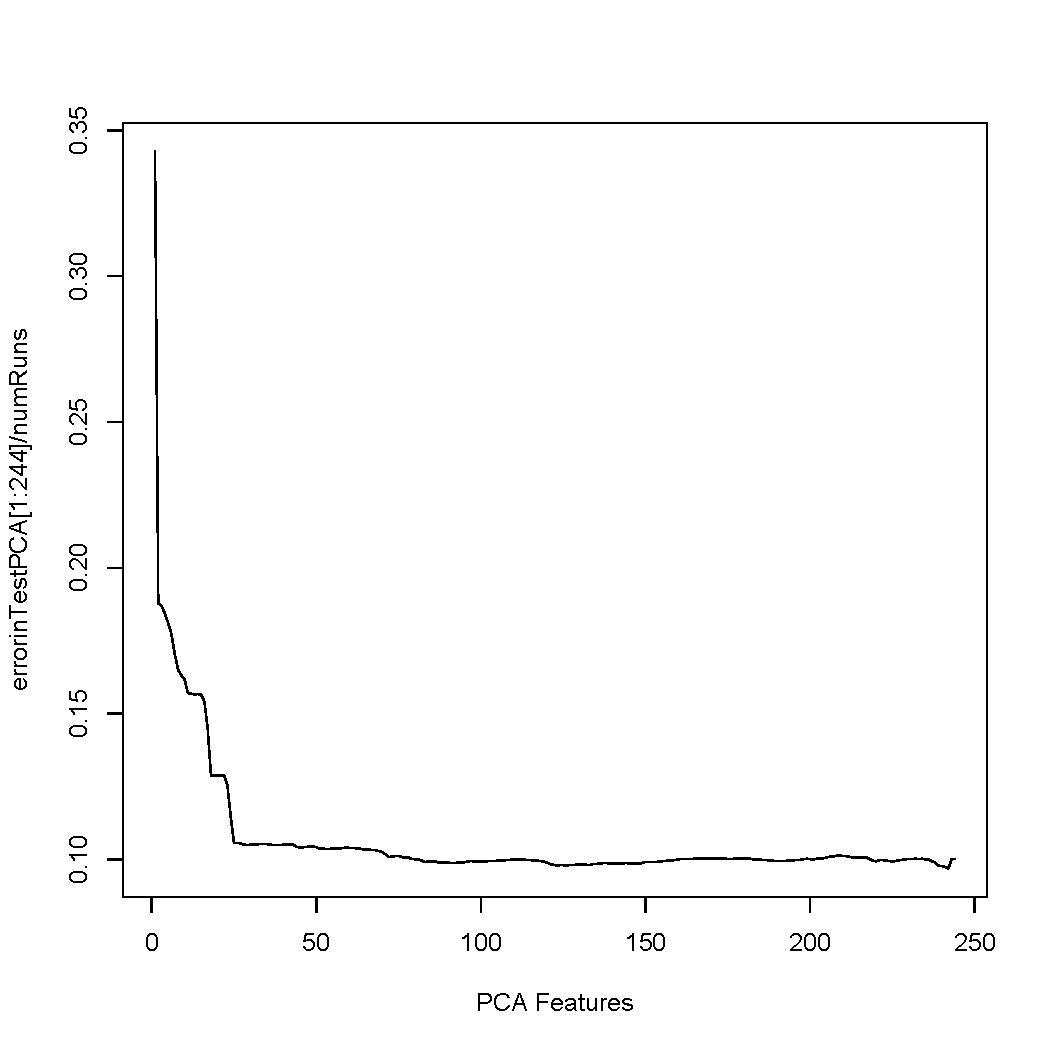
\includegraphics[scale=0.4]{PCA}
% \end{floatrow}
\caption{PCA Features}
\label{fig:cost}
\end{figure}


The experiments using clustering did not perform well and got error ranging from 100\% to 3500\%. I believe this occurred due to the lack of training samples
the clusters were comprised of. Many of the blocks only had a few points while others contained a vast majority. With more data and possibly a more carefully designed
implementation for clustering this may have performed better.




\section{Summary and Conclusions}

While this is the first step in discovering methods for predicting the sales price of houses, the above results shows promise in using data mining and machine learning techniques
for the analysis of housing data. A more reliable model using a more robust data set could be produced, but the lack of data in the set limits the amount that can be learned and
the hinders its ability to be generalized. 

Future work should go into using better methods for regression and prediction, creating and training with a larger data set to produce a more
reliable and general model, and more complex feature selection methods.  Also using a larger dataset the clustering method should be re-approached and experimented with.


%------------------------------------------------
\phantomsection
\section*{Acknowledgments} % The \section*{} command stops section numbering

We thank Indiana University, especially Prof. Dalkilic, for their gracious and unwavering commitment to students, and the Lindley Hall staff for the amazing facilities (especially the coffee machine).
Finally, we must thank the knowledgable and helpful AIs, and the omnipotent and omniscient Google.


\addcontentsline{toc}{section}{Acknowledgments} % Adds this section to the table of contents



%----------------------------------------------------------------------------------------
%	REFERENCE LIST
%----------------------------------------------------------------------------------------
\phantomsection
\bibliographystyle{unsrt}
\bibliography{report}

%----------------------------------------------------------------------------------------

\end{document}
